%
\documentclass[12pt]{article}

% The usual packages
\usepackage{fullpage}
\usepackage{breakcites}
\usepackage{setspace}
\usepackage{endnotes}
\usepackage{float}
\usepackage{amsmath}
\usepackage{amsfonts}
\usepackage{amssymb}
\usepackage{rotating}
\usepackage{longtable}
\usepackage{microtype}
\usepackage{graphicx}
\usepackage{hyperref}
%\usepackage[usenames,dvipsnames]{color}
\usepackage{url}
\usepackage{natbib}
\usepackage{framed}
\usepackage{epigraph}
\usepackage{lipsum}
\usepackage[font=small,labelfont=sc]{caption}
\restylefloat{table}
\bibpunct{(}{)}{;}{a}{}{,}

% Set paragraph spacing the way I like
\parskip=0pt
\parindent=20pt

% Define mathematical results
\newtheorem{lemma}{Lemma}
\newtheorem{proposition}{Proposition}
\newtheorem{theorem}{Theorem}
\newtheorem{claim}{Claim}
\newenvironment{proof}[1][Proof]{\begin{trivlist}
\item[\hskip \labelsep {\bfseries #1}]}{\end{trivlist}}
\newenvironment{definition}[1][Definition]{\begin{trivlist}
\item[\hskip \labelsep {\bfseries #1}]}{\end{trivlist}}
\newenvironment{example}[1][Example]{\begin{trivlist}
\item[\hskip \labelsep {\bfseries #1}]}{\end{trivlist}}
\newenvironment{remark}[1][Remark]{\begin{trivlist}
\item[\hskip \labelsep {\bfseries #1}]}{\end{trivlist}}
\DeclareMathOperator*{\argmin}{arg\,min}
\DeclareMathOperator{\med}{med}


% Set up fonts the way I like
\usepackage{tgpagella}
\usepackage[T1]{fontenc}
\usepackage[bitstream-charter]{mathdesign}

\newcommand{\specialcell}[2][c]{%
  \begin{tabular}[#1]{@{}c@{}}#2\end{tabular}}


%% Set up lists the way I like
% Redefine the first level
\renewcommand{\theenumi}{\arabic{enumi}.}
\renewcommand{\labelenumi}{\theenumi}
% Redefine the second level
\renewcommand{\theenumii}{\alph{enumii}.}
\renewcommand{\labelenumii}{\theenumii}
% Redefine the third level
\renewcommand{\theenumiii}{\roman{enumiii}.}
\renewcommand{\labelenumiii}{\theenumiii}
% Redefine the fourth level
\renewcommand{\theenumiv}{\Alph{enumiv}.}
\renewcommand{\labelenumiv}{\theenumiv}
% Eliminate spacing around lists
\usepackage{enumitem}
\setlist{nolistsep}

% Create footnote command so that my name
% has an asterisk rather than a one.
\long\def\symbolfootnote[#1]#2{\begingroup%
\def\thefootnote{\fnsymbol{footnote}}\footnote[#1]{#2}\endgroup}

% Create the colors I want
\usepackage{color}
\definecolor{darkred}{RGB}{100,0,0}

\hypersetup{
pdftitle={The Heavy Tails of Electoral Data}, % title
pdfauthor={Dan Baissa and Carlisle Rainey}, % author
pdfkeywords={robust linear regression} {outliers} {leverage}
pdfnewwindow=true, % links in new window
colorlinks=true, % false: boxed links; true: colored links
linkcolor=darkred, % color of internal links
citecolor=darkred, % color of links to bibliography
filecolor=darkred, % color of file links
urlcolor=darkred % color of external links
}

% enable comments in pdf
\newcommand{\kelly}[1]{\textcolor{blue}{#1}}
\newcommand{\carlisle}[1]{\textcolor{magenta}{#1}}


\begin{document}

\begin{center}
{\LARGE \textbf{The Heavy Tails of Electoral Data}}\\\vspace{2mm}
{ \textbf{The Importance of Robust Estimators}\symbolfootnote[1]{We thank Bill Clark and Matt Golder for making their data available to us. The analyses presented here were conducted with \texttt{R} 3.1.0. All data and computer code necessary for replication are available at \href{https://github.com/carlislerainey/heavy-tails}{
github.com/carlislerainey/meaningful-inferences}
.}}\\\vspace{2mm}


\vspace{10mm}

Dan Baissa\symbolfootnote[2]{Dan Baissa is an M.A. student in the Department of Political Science, University at Buffalo, SUNY, 520 Park Hall, Buffalo, NY 14260 (\href{mailto:dkbaissa@buffalo.edu}{
kellymcc@buffalo.edu}
).}

\vspace{3mm}

Carlisle Rainey\symbolfootnote[3]{Carlisle Rainey is Assistant Professor of Political Science, University at Buffalo, SUNY, 520 Park Hall, Buffalo, NY 14260 (\href{mailto:rcrainey@buffalo.edu}{
rcrainey@buffalo.edu}
).}
\end{center}

\vspace{10mm}

% Abstract
{\centerline{\textbf{Abstract}}}
\begin{quote}\noindent
Researchers studying the consequences of comparative electoral institutions, as well as other areas of political and social science, often estimate linear regression models on continuous outcomes of interest using least squares. These outcomes include measures of the number of political parties, proportionality, and vote share, among others. While it is well known that least-squares estimates are often sensitive to single, influential data point, this knowledge has not led to appropriate practices when using least-squares estimators. We highlight the important using more robust estimators (at least as a robustness check) and discuss several approaches to detect, summarize, and communicate the influence of particular data points. We conclude with a reanalysis of Clark and Golder (2006) an show that their conclusions depend on several influential data points. Removing these data or using a robust estimator substantially weaken their key conclusions about the conditional relationship between social heterogeneity and electoral rules in influencing the number of political parties.
 \end{quote}

% Add quote to first page
% \epigraph{}

%\begin{center}
%Manuscript word count: 
%\end{center}

% Remove page number from first page
\thispagestyle{empty}

% Start main text
\newpage
\doublespace

\section*{Introduction}

Our goal in this manuscript, our goals are to (1) highlight powerful, robust alternatives to least-squares estimators, (2) provide concrete, practical advice to substantive researchers using linear models, and (3) provide a compelling example that shows the importance of robust estimators.

\section*{Is a BLUE Estimator the ``Best'' Estimator?}

The linear regression model can be written as $E(y | X) = X\beta + \epsilon$, where $y$ is an outcome variable of interest (usually roughly continuous), $X$ is a $n \times (k + 1)$ matrix containing a single column of ones and $k$ columns holding $k$ explanatory variables, $\beta$ is a $(k + 1) \times 1$ matrix of model coefficients, and $\epsilon$ is an $n \times 1$ matrix of errors. Researchers in political science commonly estimate this model with ordinary least squares (OLS) by minimizing the squared residuals, $\hat{\beta}^{OLS} = \argmin S(b)$, where $S(b) = \sum_{i = 1}^n(y_i - X_ib)^2$. That is, OLS estimators choose the estimate $\hat{\beta}$ that minimizes the sum of the squared residuals. Under the assumption that the errors $\epsilon_i$ follow independent and identical normal distributions with mean zero and unknown variance, the OLS estimator is the minimum variance unbiased estimator (MVUE).

Even if the errors do not follow independent and identical normal distributions, the Gauss-Markov Theorem guarantees the least-squares estimator is the best (i.e., minimum variance) \textit{linear} unbiased estimator if the errors have mean zero and constant (and finite) variance. However, this should provide little comfort to researchers because their is little statistical or substantive reason to restrict themselves to \textit{linear} estimators.

At first glance, one might take the linearity restriction under Gauss-Markov to refer to the structure of the model, such that $E(y | X) = X\beta$ falls into the class of ``linear'' regression models, but  $E(y | X) = e^{X\beta}$ does not. Indeed, this is the sense in which we use ``linear'' in the term ``linear regression.'' However, the ``linear'' restriction in the Gauss-Markov Theorem refers to a highly technical and obscure statistical criterion that requires that the estimates be a linear function of the outcome variables, so that $\hat{\beta}_j = \lambda_1 y_1 + \lambda_2 y_2 + ... \lambda_n y_n$, so that the weights $\lambda_i$ are allowed to depend on $X$, but not on $y$.\footnote{Formally, linearity requires that $\hat{\beta} = My$, where $M$ depends on the matrix $X$. For the case of least-squares, $M = (X'X)^{-1}X'$.} In other words, Gauss-Markov does not require a linear \textit{model} of the form $E(y | X) = X\beta$, but it does require a linear estimator of the form $\hat{\beta}_j = \lambda_1 y_1 + \lambda_2 y_2 + ... \lambda_n y_n$. 

We can see that the least-squares criterion produces a linear \textit{estimator} with some simple algebra. First, recall that we wish to minimize $S(b) = \sum_{i = 1}^n(y_i - X_ib)^2$ w.r.t. $b$. To do this, we can simply set $\dfrac{\partial S(b)}{\partial b} \equiv 0$ and solve for the vector $b$. Noting that $\dfrac{\partial S(b)}{\partial b} = \sum_{i = 1}^n 2(y_i - X_ib)(-X_i) \equiv 0$ implies that $\sum_{i = 1}^n X_i(y_i - X_ib) \equiv 0$. This is simply a system of $k+1$ \textit{linear} equations $\sum_{i = 1}^n X_{ij}(y_i - X_ib)$ for $k = \{0, 1, 2,..., k\}$. Of course, the matrix form $X'(y - Xb) = 0 \Rightarrow (X'X)b = X'y \Rightarrow b = (X'X)^{-1}X'y$ is much more common. We can clearly see that the least squares estimator $\hat{\beta}^ls = (X'X)^{-1}X'y$ has the form $My$.

However, we argue that restricting ourselves to linear estimators is unnecessary and unproductive. Note that we are not arguing against linear models (i.e., models that are linear in the parameters), such $y_i = \beta_0 + \beta_1\sqrt(x_i) + \epsilon_i$, $y_i = \beta_0 + \beta_1x_i + \beta_2x_i^2 + \epsilon_i$,  or $y_i = \beta_0 + \beta_1x_i + \beta_2z_i + \beta_3x_iz_i + \epsilon_i$. Indeed, the linear model can represent a wide range of theoretically-relevant relationships, especially when it includes explanatory variables non-linearly. However, there is no statistical reason to restrict ourselves to linear \textit{estimators}, except for mathematical convenience, and there are substantive reasons to reject this restriction. For example, if the researcher is aware that one case has a unusually large outcome variable (conditional on the explanatory variables), then the researcher might wish to weight that case less than the other, more typical cases so that one atypical case does not exert several times more impact on the estimates than other, typical cases. Indeed, substantive researchers might wish to attach zero weight to extremely unusual cases because these cases might be due to a different substantive process.

\section*{A Substantive Argument Against Linear Estimators}

Indeed, there is a substantive argument \textit{against linear estimators} (i.e., weighting all observations equally). We suggest two potentially desirable properties of estimators. First, we might like estimates that provide an excellent fit to \textit{most} of the data rather and a poor fit to some of the data, rather than a mediocre fit to \textit{all} the data. Secondly, we might prefer an estimate that treats unusual data equally--as inconsistent the the model. Either of these principles exclude linear estimators.

For example, consider the estimates shown in the left panel of Figure \ref{fig:best-fit-illustration}. Which of the two estimates, A or B, best summarizes the relationship between the explanatory and outcome variable? Estimate A fits all the data decently, but estimate B provides an excellent summary for most of the data. Which is preferred? At least in some cases, we might prefer estimate B because we wish to discount the three unusual cases as inconsistent with the model (perhaps these cases are elections marred with scandals, etc.).

\begin{figure}[H]
\begin{center}
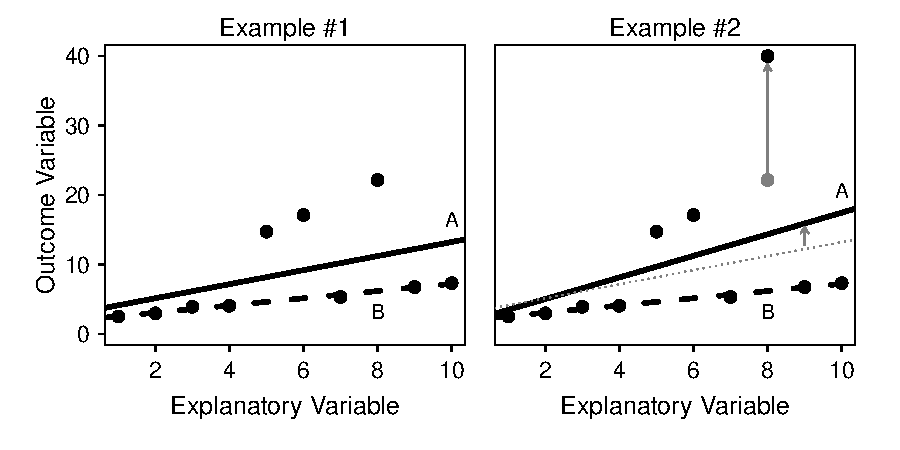
\includegraphics[scale = .7]{figs/best-fit-illustration.pdf}
\caption{caption here}\label{fig:best-fit-illustration}
\end{center}
\end{figure}

Secondly, once cases fall outside the explanatory power of the model (i.e., outliers), then we might like our estimators to give them zero weight. After all, these cases seem somehow different and we would not like these unusual data to affect our excellent fit for the majority of the data. That is, if one unusual cases was \textit{even more} unusual, the estimates should not change. Rather than respond to this unusual deviation as does estimate A, we might prefer an estimate that simply ignores this change. After all, the case seems to fall outside the explanatory power of the model in both cases.



It is not often appreciated that if the errors do not follow independent and identical normal distributions, then the OLS is no longer the MVUE--other estimators might outperform OLS.

Many researchers simply assume a statistical model for which a MVUE is easily available for little or no substantive reason. Knowing that the assumed model (e.g., normality) is \textit{in}orrect, these researchers are using this model as an approximation. But if the model is an approximation, then the desirable statistical properties are not longer guaranteed (e.g., MVUE). With this in mind, it makes more sense to use a robust estimator with the following qualitative properties:
\begin{enumerate}
\item Approximately unbiased in typical sample sizes for the assumed model and small, plausible deviations.
\item Excellent efficiency under the assumed model, though perhaps not the best possible efficiency.
\item Excellent efficiency under small deviations from the assumed model
\item Reasonable efficiency and bias in typical sample sizes with large deviations from the assumed model. 
\end{enumerate}

Mathematically, this suggests that applied researchers should not necessarily restrict themselves to unbiased estimators or minimum variance estimators under an assumed model. Instead, a more desirable criterion might be the mean squared error of the estimate under a wide range of deviations from the assumed model. The ``best'' model for a social scientist might not be the optimal estimator for an assumed model, but an estimable that works reasonably well for the assumed model and many substantively plausible deviations. 

To see the importance of this in practice, we simulated 10,000 data sets 50 observations of variables $x$ and $y$, where the relationship between $x$ and $y$ is given by $y = x + \epsilon$, where $\epsilon$ follows a $t$ distribution with three degrees of freedom. Note that the $t_3$ distribution is symmetric, bell-shaped, and resembles the normal distribution, except it has slightly heavier tails. For each of these 10,000 data sets we used least-squares to estimate the slope of the relationship between $x$ and $y$. Because we simulated these data, we know that the Gauss-Markov assumptions hold. This means that least-squares is the \textit{best} linear unbiased estimator. The left panel of Figure \ref{fig:lts-illustration} shows the distribution of the estimated slopes using least squares.

But consider a least trimmed squares (LTS) estimator in which we minimize the smallest 90\% of the residuals. This method literally throws away data. Though it lacks the elegant theory of the least-squares estimate, the right panel of Figure \ref{fig:lts-illustration} shows that it is essentially unbiased and, compared to the least-squares more efficient (standard deviation about 18\% smaller), and has a much smaller mean squared error (about 32\% smaller) . By any reasonable standard, it is a better estimator than the least squares estimator. This improvement is dropped by expanding our focus to non-linear estimators. In this case, the LTS estimator is not linear because it places zero weight on the largest 10\% of the residuals and weights of one on the smallest 90\% of the residuals.

\begin{figure}[H]
\begin{center}
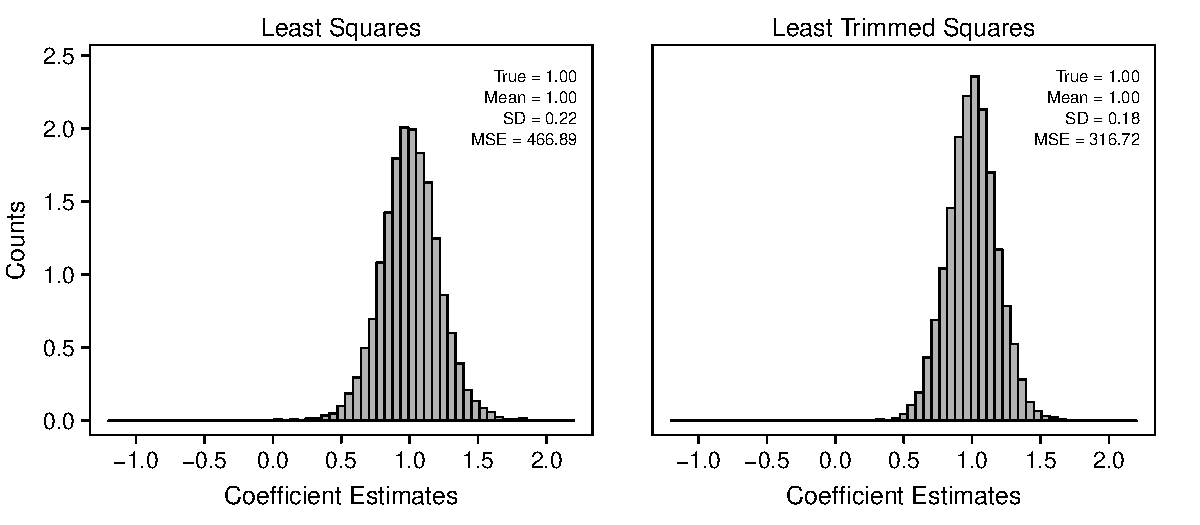
\includegraphics[scale = .7]{figs/lts-illustration.pdf}
\caption{caption here}\label{fig:lts-illustration}
\end{center}
\end{figure}

While the statistical properties of the least squares under the assumed normal-linear model are extremely well developed (e.g., MVUE), these properties are not nearly as well developed from robust alternatives. Some asymptotic results are available, but the closed-form theory is generally much weaker.

There has been a great deal of attention in the methodological literature to the sensitivity of standard errors to violations from the assumed model--and substantive scholars have paid attention. For example, White's (1980) seminal paper developing heteroskedasticity-consistent standard errors has received over 20,000 citations, making it one of the most cited papers in economics. Beck and Katz's (1995) introduction to panel corrected standard errors has received over 4,300 citations, making it one of the most cited political science papers ever.

On the other hand, there has been scant attention paid to the sensitivity of the estimates to similar violations. This is particularly problematic, since it makes little sense to find a good standard error for a poor estimate. Two papers in political science have addressed the issue of robust estimation. Western's (1995) introduces political scientists to robust estimators, but this work has been essentially ignored. The work is more broadly applicable than Beck and Katz (1995) and was published in the same year, but has received only 99 citations, or  about 2\% of the citations that Beck and Katz have received. Similarly, Demaris and Harden (2011) has received only one citation, and it comes from the authors themselves. Anderson's (2008) broad and accessible introduction to robust estimation methods has received only about 150 citations, most from outside political science.

This focus on obtaining reasonable standard errors at the expense of reasonable estimates can be seen in Gujarati (????, p. ??, ), a popular textbook for political science classes focusing on linear models. Though the text deals with robust standard errors in some detail, Gujarati writes (in a footnote):
\begin{quote}
In passing, note that the effects of departure from normality and related topics are often discussed under the topic of robust estimation in the literature, a topic \textit{beyond the scope of this book} [italics ours].
\end{quote}
Another popular textbook, Wooldridge (????) does briefly discuss robust estimators, though in a much more limited manner than his discussion of robust standard errors. Angrist and Pischke (2008), though, devote an entire chapter to robust standard errors and completely ignore robust estimation of model coefficients.

\section*{Dealing with Skewness: Transforming the Outcome}

Skewed error distribution create two problems for the linear model. First, because least squares models the quantity $E(Y | X)$ and the mean is not a good summary of location for skewed variables. Symmetric error distributions are easier to understand. Second, and perhaps most importantly, we take skewed error distributions as a lack of model fit. For example, it is theoretically intuitive to believe that the explanatory variables should have increasing effects non-negative outcome variables, such as an individual's annual income. For example, rather than a college degree increasing one expected income by \$10,000, perhaps it increases one's expected income by 10\%. We consider skewed error distributions as evidence that the basic structure of the model could be improved.

Points that are unusual prior to transformation might be quite typical after transformation.

Even if we remain indifferent toward the theoretical implications of skewed error distributions, we must remain cautious about the statistical implications. The performance of least squares estimators improves as the error distribution approaches a normal distribution. Further, the theoretical properties of alternative, more robust estimators, such as the $M$-estimator we discuss below, depend on a symmetric error distribution distribution.

It is quite common in disciplines such as economics, for example, to log-transform non-negative outcome variables by default. The motivation is that since non-negative (or strictly positive) outcomes are bounded below by zero, then these variables are likely skewed to the right. In this case, the model $\log(y) = X\beta + \epsilon$ will likely provide a better approximation to the data.

While we agree with the spirit of this suggestion, we have much more precise empirical methods for choosing \textit{whether} and \textit{how} to transform the outcome variable $y$. Box and Cox (1964) proposed the Box-Cox transformation 

\begin{displaymath}
   y^{(\lambda)} = BC(y, \lambda) = \left\{
     \begin{array}{lr}
       \dfrac{y^\lambda - 1}{\lambda} & \text{for } \lambda \neq 0\\
       \log y & \text{for } \lambda \neq 0
     \end{array}
   \right.
\end{displaymath}.

\noindent In this case, the model becomes $y^{(\lambda)} = X\beta + \epsilon$. The researcher can easily use maximum likelihood to obtain estimates $\hat{\lambda}$ and standard errors for the transformation parameter $\lambda$. This is particularly convenient because if $\hat{\lambda}$ is near one, this suggests no transformation is needed and if $\hat{\lambda}$ is near zero, then only an intuitive log-transformation is needed.

It is quite easy to assess the skewness in the residuals using a simple histogram of the residuals or a QQ plot of the residuals compared to their normal quantiles. For a formal test of skewness, one might use a direct test for symmetry on residuals $\hat{e}$, such as the Mira test (Mira 1999) or simply test whether $\lambda \neq 1$ under the Box-Cox framework. However, the important point is not to argue for any particular test, but to point out (1) that asymmetries worsen the performance of least squares and alternative methods and (2) this potential problem can and should be addressed using simple transformations that are easy to implement.

However, applying transformation to the outcome variable $y$ does raise an interpretational difficulty. The usual, untransformed linear model is given by $y = X\beta + \epsilon$ and the quantity of interest is $E(y | X)$ or $\frac{\partial E(y | X)}{\partial x_j}$. For concreteness, consider the log-transformation. Using the same logic, then the model is $log(y) = X\beta + \epsilon$ and we might take the quantity of interest to be $E[\log(y) | X]$ or $\frac{\partial E[\log(y) | X]}{\partial x_j}$. However, these quantities are not as easy to understand substantively--$\frac{\partial E[\log(y) | X]}{\partial x_j}$ is more difficult to understand than $\frac{\partial E(y | X)}{\partial x_j}$. To make the results more understandable, we simply need to ``undo'' the transformation. However, it is important to note that $E[\log(y) | X] \neq \log [E(y | X)]$, which means that the log cannot simply be undone (without additional computation) because $e^{E[\log(y) | X]} \neq E(y | X)$. 

However, in the context of skewed distributions, the mean $E(\dot)$ might be a misleading summary of the ``center'' of the data. While the mean is often more mathematically convenient, the median offers a better summary of location than the mean. Further, the median has an intuitive interpretation because there is a one-half of the distribution lies above the median and one-half lies below. This mean that there is approximately a one-half chance that $y |X$ falls above $\med(y | X)$ and a one-half changes that $y |X$ falls below.

In addition to the intuitive substantive interpretation of $\med(y | X)$, the median has another desirable property. Because the log-transformation is order-preserving $\med[\log(y) | X] = \log [\med(y | X)]$, which means that the log \textit{can} easily be undone because $e^{med[\log(y) | X]} = e^{\log[\med(y | X)]} = \med(y | X)$. Therefore, by adopting $\med(y | X)$ and $\frac{\partial \med(y | X)}{\partial x_j}$, one gains a more intuitive quantity of interest and can easily move between transformed and untransformed outcomes (e.g., $\med[\log(y)] \rightarrow \med(y)$). This holds for the more general case of $y^{(\lambda)}$ in addition to $\log(y)$.

To obtain quantities of interest for $\med(y)$ when the estimated model has the generic form $y^{(\lambda)} = X\beta + \epsilon$, one can simply use the algorithm described in King, Tomz, and Wittenberg (2000).
\begin{enumerate}
\item Estimate the model $y = X\beta + \epsilon$ using least squares to obtain the estimated model coefficients $\hat{\beta}^{ls}$ and residuals $\hat{e}^{ls}$. Evaluate whether the assumption of the normal errors matches the estimated residuals using histograms and QQ plots.
\item If needed, estimate the Box-Cox transformation parameter $\hat{\lambda}$ using maximum likelihood. (If the values one or zero fall within the confidence interval, then one may wish to use those values to maintain the direct interpretability of the model coefficients.)
\item Estimate the transformed model $y^{(\lambda)} = X\beta + \epsilon$ using least squares to obtain the estimated model coefficients $\hat{\beta}^{ls}_{trans}$, residuals $\hat{e}^{ls}_{trans}$, and covariance matrix $\Sigma^{ls}_{trans}$.
\item Choose a hypothetical case or set of cases $X_{pred}$ for which to calculate the quantity of interest. If one is interested in calculating a first difference, it is convenient to use $X_{hi}$ and $X_{lo}$, where the first-difference $\Delta(y, X_{hi}, X_{lo}) = \med(y | X_{hi}) - \med(y | X_{lo})$.
\item Following King, Tomz, and Wittenberg (2000), for $i$ from one to a large (e.g., 1,000) number of iterations $n_{sims}$:
	\begin{enumerate}
	\item Simulate $\tilde{\beta}^{ls}_{trans} \sim N\left(\hat{\beta}^{ls}_{trans}, \Sigma^{ls}_{trans}\right)$.
	\item Calculate and store $\tilde{Q}_i = \med(y | X_{red}, \tilde{\beta}^{ls}_{trans}) = X_{red}\tilde{\beta}^{ls}_{trans}$ or, if interested in the first-difference, $\tilde{Q}_i = \tilde{\Delta}(y, X_{hi}, X_{lo}, \tilde{\beta}^{ls}_{trans}) = X_{hi}\tilde{\beta}^{ls}_{trans} - X_{lo}\tilde{\beta}^{ls}_{trans}$.
	\end{enumerate}
\item Summarize the $n_{sims}$ simulations. The mean or median of $\tilde{Q}_i$ serves as an estimate of $\med(y | X_{pred})$, the standard deviation of $\tilde{Q}_i$ serves as an estimate of the standard error of $\med(y | X_{pred})$, and the 5th and 95th percentiles of $\tilde{Q}_i$ serve as an estimate of the (likely asymmetric) 90\% confidence interval for $\med(y | X_{pred})$.
\end{enumerate}

\section*{Dealing with Heavy-Tails: $M$-Estimation}

In spite of the scant attention paid to robust estimators in political science, statisticians have developed and refined many robust methods since the seminal work of Box (1953) and Huber (1964). Huber and Ronchetti (2009) provide a detailed review of these developments and Anderson (2008) provides an accessible introduction. 

Adjudicating among these many robust alternatives to least squares is beyond the scope of our paper, but, to fix ideas, we do introduce one robust estimator in detail which has several desirable properties--the $M$-estimator with Tukey's biweight function. 

While least squares yields the coefficients that minimize the sum of the squared residuals, so that $\hat{\beta}^{ls} =\argmin_{b} \sum_{i = 1}^n (y_i - X_ib)^2$, M-estimation minimizes an arbitrary, less-rapidly increasing function of the residuals $\hat{\beta}^{\rho} =\argmin_{b} \sum_{i = 1}^n \rho(y_i - X_ib)$. For example, Harden and Desmarais (2011) recommend the least absolute deviation (LAD) estimator that chooses $\rho(\dot) = abs(\dot)$. However, other estimators offer similarly robust alternatives. In particular, we recommend Tukey's biweight function, so that

\begin{displaymath}
   \rho_{bw}(r_i) = \left\{
     \begin{array}{lr}
       \dfrac{k^2}{6}\left\{ 1 - \left[ 1 - \left( \dfrac{r_i}{k} \right)^2 \right]^3\right\} & \text{for } |r_i| \leq k\\
	\dfrac{k^2}{6} & \text{for } |r_i| > k 
\end{array}
   \right.,
\end{displaymath}.

where $r_i = y_i - X_ib$.

[Discuss the desirable substantive properties of bw, such as fitting the majority of the data well and ignoring, rather than simply down weighting unusual data.]

Two cautions are in order. Second, the optimization problem is not convex, so standard optimization routines can produce a local rather than a global minimum. Second, because the solution is not scale invariant, the residuals $\hat{e_i}$ are standardized by a robust estimate of scale $\hat{\sigma}_{(mad)}$, which must of course be estimated jointly, so that $\hat{\beta}^{bw} =\argmin_{b} \sum_{i = 1}^n \rho_{bw}\left(\dfrac{y_i - X_ib}{\hat{\sigma}_{mad}}\right)$, where $\hat{\sigma}_{mad} = \dfrac{\med\left( |y - X\b|\right)}{0.6745}$. Dividing by 0.6745 makes $\hat{\sigma}_{mad}$ a consistent estimator of the standard deviation of normal errors.

The model parameters $\hat{\beta}^{bw}$ and $\hat{\sigma}_{bw}$ can be quickly estimated jointly using the following iterative algorithm.
\begin{enumerate}
\item Start with initial estimate of the coefficients $\hat{\beta}^{(0)}$. The choice of initial estimator is not trivial. In the case of extreme outliers and/or many parameters, starting with least squares might lead the algorithm to a local minimum. We recommend the least trimmed squares method discussed earlier to obtain starting values.
\item Extract the residuals $r^{(0)} = X\hat{\beta}^{(0)}$. Use these residuals to estimate the rescaled MAD so that $\hat{\sigma}^{(0)}_{mad} = \dfrac{\med\left( |y - X\hat{\beta}^{(0)}|\right)}{0.6745}$.
\item ssign weights $w$ according to the function $\rho$ and denote $\text{diag}(w) = W$.
\item For $i$ from one until convergence:
	\begin{enumerate}
	\item Using $\hat{\beta}^{(i-1)}$ and $\hat{\sigma}^{(i-1)}_{mad}$ assign weights $w$ according to the function $\rho$ and denote $\text{diag}(w) = W$.
	\item Calculate $\hat{\beta}^{(i)} = (X'WX)^{-1}X'Wy$.
	\item Calculate $\hat{\sigma}^{(i)}_{mad} = \dfrac{\med\left( |y - X\hat{\beta}^{(0)}|\right)}{0.6745}$
	\item The algorithm has converged when $r^{(i-1)} \approx r^{(i)}$.
	\end{enumerate}
\end{enumerate}

[Discuss some properties of M-estimators, unbiased for symmetric error distributions, consistent.]

[Discuss standard errors for m-estimators.]

\section*{Monte Carlo Simulations}

To understand and illustrate how the performance of the biweight $M$-estimator, we simulated from the linear model $y_i = \beta_0 + \beta_1x_1 + \beta_2 x_2 + \beta_3 x_3 + \epsilon_i$, where $\beta_0 = 0$ and $\beta_1 = \beta_2 = \beta_3 = 1$ and the $x_i$'s follow an approximately normal distribution. We used four different distribution for the errors.
\begin{itemize}
\item \textit{Laplace distribution.} The Laplace distribution has tails that decrease exponentially, but behaves much differently from the normal distribution near zero. Rather than ``shoulders,'' the Laplace distribution has a sharp peak at zero and can be thought of as combining two exponential distributions, one in the positive direction and the other in the negative direction. The least absolute deviation estimator is the maximum likelihood estimator when the errors follow a Laplace distribution.
\item \textit{$t_2$ distribution.} The $t$ distribution with two degrees of freedom has very heavy tails. Because the least squares estimator weights all points equally (conditional on $X$), the extreme outliers produces by the $t_2$ distribution makes least squares a very inefficient estimator.
\item \textit{$t_{10}$ distribution.} The $t$ distribution with ten degrees of freedom has slightly heavier tails than the normal distribution. The $t_10$ distribution has \textit{slightly} heavier tails than the normal distribution. To get a sense for just how similar a $t_{10}$ distribution is to a normal distribution, note that a Shapiro-Wilk test of normality only successful rejects the null in about 65\% of repeated samples if 500 observation are simulated from a $t_{10}$ distribution.\footnote{One needs about 750 samples to reach 80\% power.} It is essentially impossible to spot the differences between the normal and $t_{10}$ density functions without plotting the two directly on top of each other, in which case the $t_{10}$ has \textit{slightly} heavier tails.
\item \textit{Normal Distribution.} The normal distribution yields the optimal conditions for the least squares estimator. Indeed, when the errors follow a normal distribution, the least squares estimator is has the smallest variance of all unbiased estimators. 
\end{itemize}

For two different sample sizes, 100 and 1,000, and the four different error distributions, we simulated 10,000 data sets, estimated $\beta_1$ using the least squares estimator, the median absolute deviation estimator, and the biweight estimator. For each condition, we calculated the expected value of the estimate, the standard deviation, and the mean squared error. Table \ref{tab:tab:mc-sims-100} provides the results for the sample size of 100 and \ref{tab:tab:mc-sims-1000} provides the results for the sample size of 1,000. 

\begin{table}
{\tiny
% quantreg::latex.table(x = ta, file = "doc/tabs/mc-sims-100",      rowlabel = "", cgroup = c("Mean", "Standard Deviation", "Mean Squared Error"),      rgroup = c("Absolute Performance", "Relative Performance"),      n.rgroup = c(3, 2), dec = 3, table.env = FALSE, label = "tab:mc-sims-100") 
%
\begin{center}
\begin{tabular}{|l||c|c|c|c||c|c|c|c||c|c|c|c|} \hline
\multicolumn{1}{|l||}{\bf }&\multicolumn{4}{c||}{\bf Mean}&\multicolumn{4}{c||}{\bf Standard Deviation}&\multicolumn{4}{c|}{\bf Mean Squared Error}\\ \cline{2-13}
\multicolumn{1}{|l||}{}&\multicolumn{1}{c|}{Lapl.}&\multicolumn{1}{c|}{$t_2$}&\multicolumn{1}{c|}{$t_{10}$}&\multicolumn{1}{c||}{Norm.}&\multicolumn{1}{c|}{Lapl.}&\multicolumn{1}{c|}{$t_2$}&\multicolumn{1}{c|}{$t_{10}$}&\multicolumn{1}{c||}{Norm.}&\multicolumn{1}{c|}{Lapl.}&\multicolumn{1}{c|}{$t_2$}&\multicolumn{1}{c|}{$t_{10}$}&\multicolumn{1}{c|}{Norm.}\\ \hline
{\bf Absolute Performance}&&&&&&&&&&&&\\
~~Least Squares&~~~0.999&~~~1.000&~~~1.001&~~~0.999&~~~0.151&~~~0.319&~~~0.114&~~~0.099&~227.419&1016.182&~130.867&~~98.850\\ 
~~Least Absolute Deviation&~~~0.999&~~~0.999&~~~1.003&~~~1.000&~~~0.126&~~~0.146&~~~0.131&~~~0.124&~159.499&~212.360&~172.911&~154.714\\ 
~~Tukey's Biweight&~~~1.000&~~~0.999&~~~1.001&~~~0.999&~~~0.131&~~~0.138&~~~0.113&~~~0.102&~172.043&~189.519&~127.731&~104.759\\ \hline
{\bf Relative Performance}&&&&&&&&&&&&\\
~~LAD/LS&~~~1.001&~~~0.999&~~~1.002&~~~1.001&~~~0.837&~~~0.457&~~~1.149&~~~1.251&~~~0.701&~~~0.209&~~~1.321&~~~1.565\\ 
~~BW/LS&~~~1.001&~~~1.000&~~~1.000&~~~1.000&~~~0.870&~~~0.432&~~~0.988&~~~1.029&~~~0.757&~~~0.187&~~~0.976&~~~1.060\\ 
\hline
\end{tabular}
\end{center}

}
\caption{Summarizes of the Monte Carlo simulations for four different error distributions with a sample size of 100.}\label{tab:mc-sims-100}
\end{table}

\begin{table}
{\tiny
% quantreg::latex.table(x = ta, file = "doc/tabs/mc-sims-1000",      rowlabel = "", cgroup = c("Mean", "Mean Squared Error"),      rgroup = c("Absolute Performance", "Relative Performance"),      n.rgroup = c(3, 2), dec = 3, table.env = FALSE, label = "tab:mc-sims-1000") 
%
\begin{center}
\begin{tabular}{|l||c|c|c|c||c|c|c|c|} \hline
\multicolumn{1}{|l||}{\bf }&\multicolumn{4}{c||}{\bf Mean}&\multicolumn{4}{c|}{\bf Mean Squared Error}\\ \cline{2-9}
\multicolumn{1}{|l||}{}&\multicolumn{1}{c|}{Lapl.}&\multicolumn{1}{c|}{$t_2$}&\multicolumn{1}{c|}{$t_{10}$}&\multicolumn{1}{c||}{Norm.}&\multicolumn{1}{c|}{Lapl.}&\multicolumn{1}{c|}{$t_2$}&\multicolumn{1}{c|}{$t_{10}$}&\multicolumn{1}{c|}{Norm.}\\ \hline
{\bf Absolute Performance}&&&&&&&&\\
~~Least Squares&~~0.999&~~0.999&~~1.000&~~1.000&~20.173&165.585&~12.793&~~9.998\\ 
~~Least Absolute Deviation&~~1.000&~~1.000&~~1.001&~~1.000&~11.352&~19.928&~17.123&~15.867\\ 
~~Tukey's Biweight&~~0.999&~~1.000&~~1.000&~~1.000&~14.705&~18.567&~12.482&~10.523\\ \hline
{\bf Relative Performance}&&&&&&&&\\
~~LAD/LS&~~1.001&~~1.000&~~1.000&~~1.000&~~0.563&~~0.120&~~1.338&~~1.587\\ 
~~BW/LS&~~1.000&~~1.000&~~1.000&~~1.000&~~0.729&~~0.112&~~0.976&~~1.053\\ 
\hline
\end{tabular}
\end{center}

}
\caption{Summary of Monte Carlo simulations identical to those in Table Table \ref{tab:mc-sims-100}, except with a sample size of 1,000 rather than 100. }\label{tab:mc-sims-1000}
\end{table}

These result show that all three estimators are essentially unbiased regardless of the error distribution and sample size. Efficiency, however, varies considerably across the estimators.

The MAD estimator is the MLE when the errors follow a Laplace distribution, so as we might expect, the MAD performs well for Laplace errors, with a mean squared error about 30\% lower than the least squares error distribution. However, the biweight estimator also performs quite well for the Laplace distribution, with a mean squared error about 25\% less than the least squares estimator for $N = 100$. For $N = 1,000$ the MSE of the MAD estimator outperforms the LS estimator by about 43\% and the biweight estimator outperforms the LS estimator by about 27\%.

The $t_2$ distribution is nearly a worst case for the least squares estimator, so both robust alternatives perform considerably better. The MAD estimator is has a mean squared error of about 92\% less than the least squares estimator and the biweight estimator has a MSE about 93\% less than the LS estimator for $N = 100$ and 15\% and 14\% for $N = 1,000$, respectively. 

However, the $t_{10}$ distribution is a much more interesting case, because it is very similar to a normal distribution. Indeed, even statistical tests have trouble distinguishing the $t_{10}$ from the normal, even with large samples (e.g., $N = 500$). In this case, the MAD estimator has a MSE of about 34\% more than the LS estimator for $N = 100$ and about 32\% for $N = 1,000$. The biweight estimator on the other hand, shows a small \textit{improvement} over the LS estimator, with an MSE of about 2\% less than the LS estimator for $N = 100$ and about $4\%$ less for $N = 1,000$.

The normal distribution is the optimal scenario for the least squares estimator and it outperforms the the MAD estimator considerably with the errors are normal. For both $N = 100$ and $N = 1000$, the MSE for the MAD estimator is about 57\% larger than the MSE for the LS estimator. However, the biweight estimator performs nearly as well as the LS estimator. Indeed, the MSE for the biweight estimator is only about 6\% larger than the MSE for the LS estimator for both $N = 100$ and $N = 1000$.

Notice that while the biweight estimator was not the most efficient estimator for the Laplace and normal distributions, it was a close second. It was the most efficient estimator for the $t_2$ and $t_10$ distributions and considerably outperforms the LS estimator for Laplace errors and considerably outperforms the MAD estimator for normal errors. Thus, the biweight estimator works quite well across a range of error distributions, whereas the LS and MAD estimators work well only in particular situations.

To better understand how the heaviness of the tails of the error distribution affects the efficiency of these estimators, we repeated these simulates for $t$ distributions for degrees of freedom ranging from two to thirty and sample sizes 25, 100, 500, and 2,000. Figure \ref{fg:mc-sims} shows the performance of the MAD and biweight estimators relative to the LS estimtator.

\begin{figure}[h!]
\begin{center}
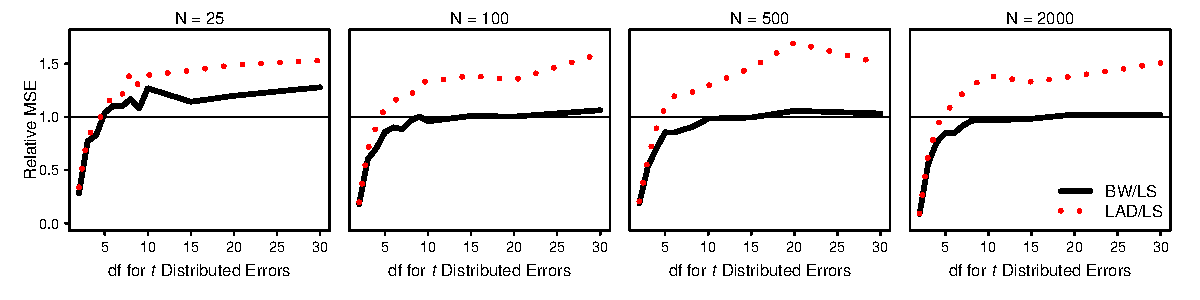
\includegraphics[width = \textwidth]{figs/mc-sims.pdf}
\caption{caption here}\label{fig:mc-sims}
\end{center}
\end{figure}

Notice that the MAD and biweight estimators perform quite well for very heavy tailed distribution (i.e., df of 2 to 4), but as the tails grow lighter, the least squares estimator quickly begins to outperform the MAD estimator. Indeed, expect of all but very heavy tailed distributions, the LS estimator is considerably more efficient than the MAD estimator. 

The biweight estimator, though, is a much stronger competitor for the least squares estimator. While the LS estimator is more efficient for lighter-tailed distributions (i.e., $df > 10$), the difference is very small except in very small samples. Indeed, for sample sizes of 100 or larger, the LS estimator is about 5\% more efficient \textit{at best}. This simulation again suggests that the biweight estimator works almost as well as the LS estimator under ideal conditions for LS estimator and considerably better across a wide range of other, substantively plausible scenarios.


\section*{Replication of Clark and Golder (2006)}

Clark and Golder (2006, p. 694) write: 

\begin{quote}
According to Duverger, the mechanical effect of electoral institutions favoring large parties creates incentives for strategic entry and strategic voting. Parties that have no chance of winning are encouraged to withdraw. If these parties fail to withdraw, then voters will have an incentive to vote strategically in favor of better placed parties. Thus disproportional systems with low district magnitudes are likely to reduce the demand for political parties created by social heterogeneity.
\end{quote}

For our replication, we focus specifically on their hypothesis:
\begin{quote}
\textsc{Hypothesis:} Social heterogeneity increases the number of electoral parties only when the district magnitude is sufficiently large.
\end{quote}

This suggests that the marginal effect of social heterogeneity should be positive and statistically significant under permissive electoral rules (i.e., large district magnitude) and about zero and statistically insignificant (though see Rainey 2014) under restrictive electoral rules (i.e., district magnitude near one).

[Summarize G and G's measures of ENEG, ENEP, and Magnitude.]

To test this hypothesis, Clark and Golder fit the following regression model using least squares:

\begin{align*}
\text{ENEP}_i = \beta_0 &+ \beta_1 \text{ENEG}_i + \beta_2 \log(\text{Magntiude}_i) + \beta_3 \text{Upper-Tier Seats}_i\\
						     &+\beta_4 \text{Presidential Candidates}_i + \beta_5 \text{Proximity}_i\\
						     &+ \beta_6 \text{Ethnic}_i \times \log (\text{Magnitude}_i) + \beta_7 \text{Ethnic}_i \times \text{Upper-Tier Seats}_i\\
						     &+ \beta_7 \text{Presidential Candidates}_i \times \times \text{Proximity}_i + \epsilon_i\text{ ,}
\end{align*}

The first key coefficient in this analysis is $\beta_1$, which summarizes the effect of social heterogeneity when district magnitude is one (i.e., the log of district magnitude is zero) and there are no upper-tier seats. According to the hypothesis, $\beta_1$ should be about zero. The second key coefficient is $\beta_6$, captures how the effect of social heterogeneity changes with the electoral rules. According to the hypothesis, $\beta_6$ should be positive, so that the effect of social heterogeneity becomes (perhaps more) positive as the district magnitude increases.

Clark and Golder use least squares to obtain their estimates of the model coefficients, but worry about their estimates of the standard errors. They write that ``[t]he crucial thing to remember is that although OLS is consistent with longitudinal data, the standard errors may be incorrect'' (p. 690). They discuss several options and ultimately settle on robust standard errors clustered by country, but demonstrate that their conclusions are robust to alternative approaches to estimating standard errors. However, they do not address the possibility of a non-normal error distribution or its potential impact on the coefficient estimates. This is especially concerning given that the effective number of electoral parties is bounded below by zero, perhaps creating an error distribution with a strong skew to the right. 

To get an initial sense of how the results might change using an alternative (perhaps more efficient) estimator, we replicated the estimates from four models in their Table 2. For these initial estimates, we make no attempt to account for the clustered nature of the data in calculating the standard errors, but do supply the usual 90\% confidence intervals to serve as a lower-bound on the uncertainty. Figure \ref{fig:cg-coef-plots} presents these estimates and confidence intervals.

\begin{figure}[H]
\begin{center}
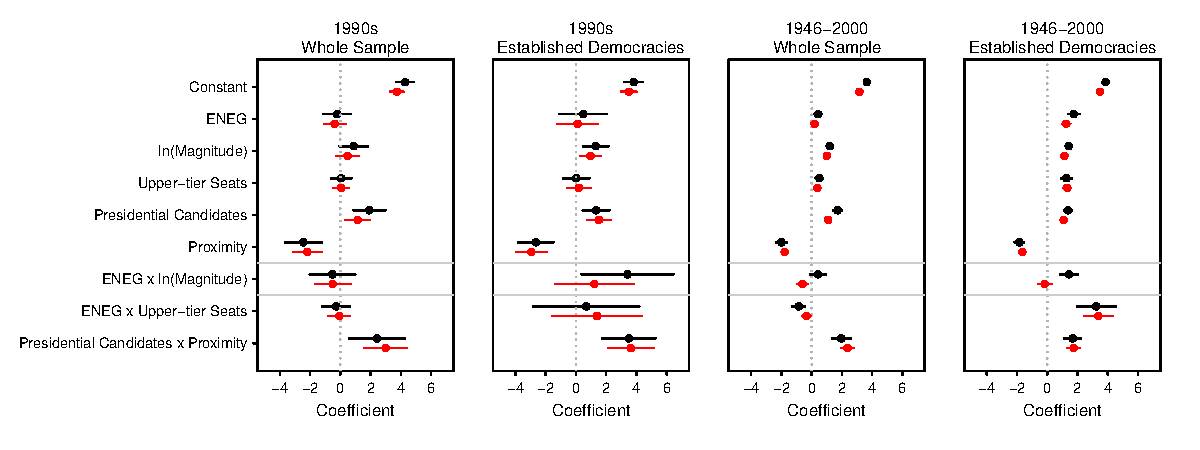
\includegraphics[scale = .8]{figs/cg-coef-plots.pdf}
\caption{Replication of Clark and Golder (2006) using MM-estimation with explanatory variables standardized to have mean zero and standard deviation one-half. The black lines and points show the OLS estimates and 90\% confidence intervals and the red lines and points show the MM estimates and confidence intervals. Notice that the coefficient for the product of the effective number of ethnic groups and the district magnitude changes drastically with the choice of estimator.}\label{fig:cg-coef-plots}
\end{center}
\end{figure}

Notice that the crucial estimate $\hat{\beta}_6$ changes substantially depending on the choice of estimator. This key estimate, which the theory suggests should be positive, remains negative in the 1990s sample including new democracies, shrinks substantially toward zero in the 1990s sample that includes only established democracies, and \textit{becomes negative} in the large sample of countries from 1946-2000 that includes new democracies \textit{and} the large sample that only includes only established democracies. These results seem to depend on the choice of estimator. In cases such as this, it is especially important to carefully examine the residuals.

For the remainder of our analysis, we focus on the estimates from large sample of countries from 1946-2000 that includes only established democracies. Figure \ref{fig:cg-residuals-hist} presents the histogram of the residuals from the least-squares estimates and Figure \ref{fig:cg-qq-plot} presents the QQ plot for these residuals. Both figures indicate a substantial skew to the right. While this does not necessarily lead to biased estimates, it does, in our view, suggest that the linear model would be more appropriate for a transformed outcome variable. If the transformation makes the errors more closely approximate a normal distribution, then the least squares estimators will be more efficient. In our view, the model for the transformed outcome can capture potentially interesting substantive effects as well.

\begin{figure}
%\centering
\begin{minipage}[t]{0.48\textwidth}
%\centering
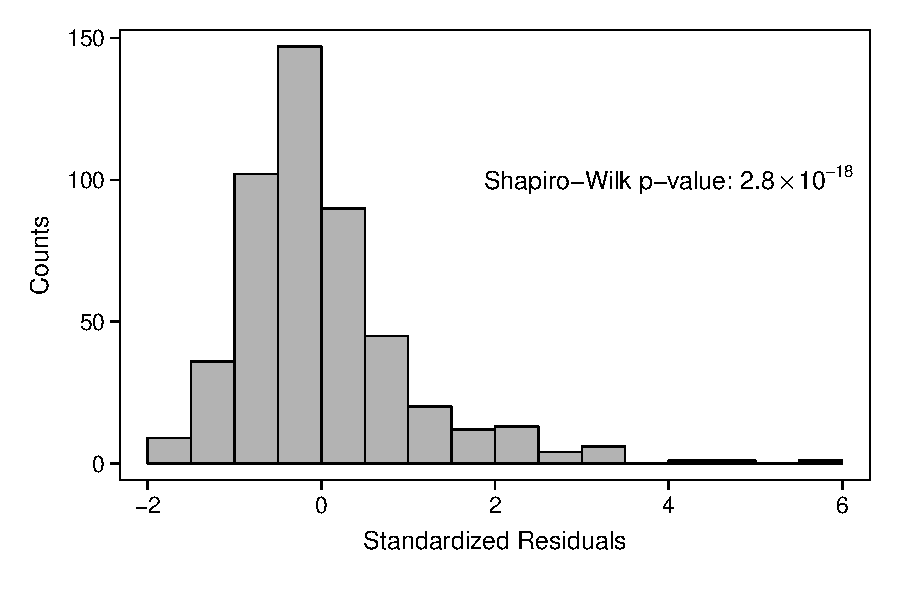
\includegraphics[width = \textwidth]{figs/cg-residuals-hist.pdf}
\caption{A histogram showing the distribution of the residuals from Clark and Golder's (2006) main model. Notice that these residuals do not seem approximately normal. They have a strong skew and heavy tail to the right. For example, one would rarely expect to observe residuals more that three standard deviations from zero if the assumption of normality holds. In these data, we have several residuals more that three standard deviations away and one nearly six standard deviations away. This suggests that some transformation of the outcome variable might be useful.}\label{fig:cg-residuals-hist}
\end{minipage}\hfill
\begin{minipage}[t]{0.48\textwidth}
%\centering
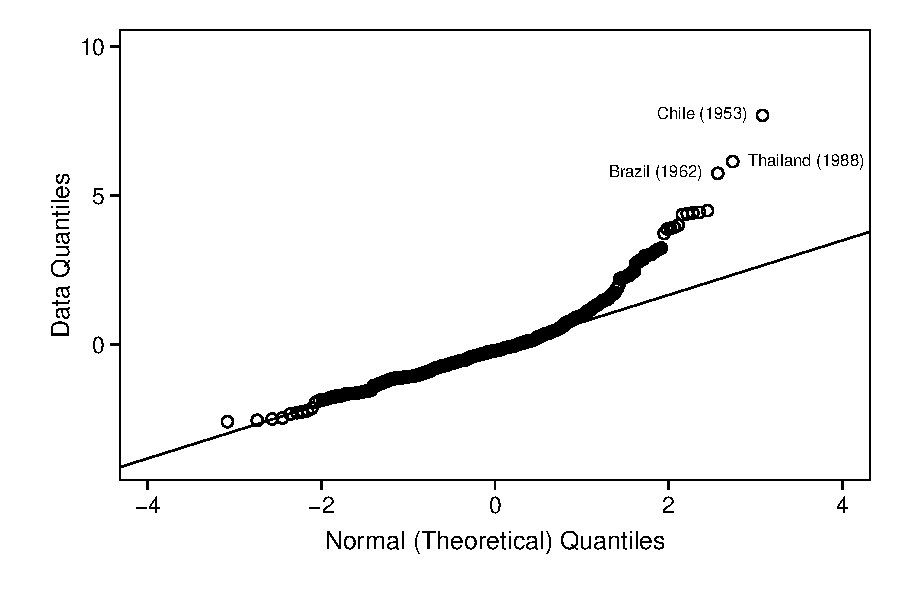
\includegraphics[width = \textwidth]{figs/cg-qq-plot.pdf}
\caption{A QQ plot showing the deviation of the residuals from normality. If the residuals were approximately normal, then the points in the QQ plot would approximately follow the line. However, notice that the positive residuals deviate sharply from the theoretical expectations. This also suggests that some transformation of the outcome variable might be useful.}\label{fig:cg-qq-plot}
\end{minipage}
\end{figure}

The maximum likelihood estimate of the Box-Cox transformation parameter $\lambda$ is about $-\frac{1}{3}$ and the confidence interval does not include zero, which suggests that a log-transformation does not quite eliminate the skew. We estimated the model using both a log-transformation and Box-Cox transformation with $\lambda = -\frac{1}{3}$. Figure \ref{ig:cg-trans-residuals-hist} present the histogram of the residuals from these two regression models. Notice that log-transforming the effective number of electoral parties does not quite remove the skew in the residuals. However, the Box-Cox transformation with $\lambda = -\frac{1}{3}$ provides highly symmetric residuals. 

\begin{figure}[h!]
\begin{center}
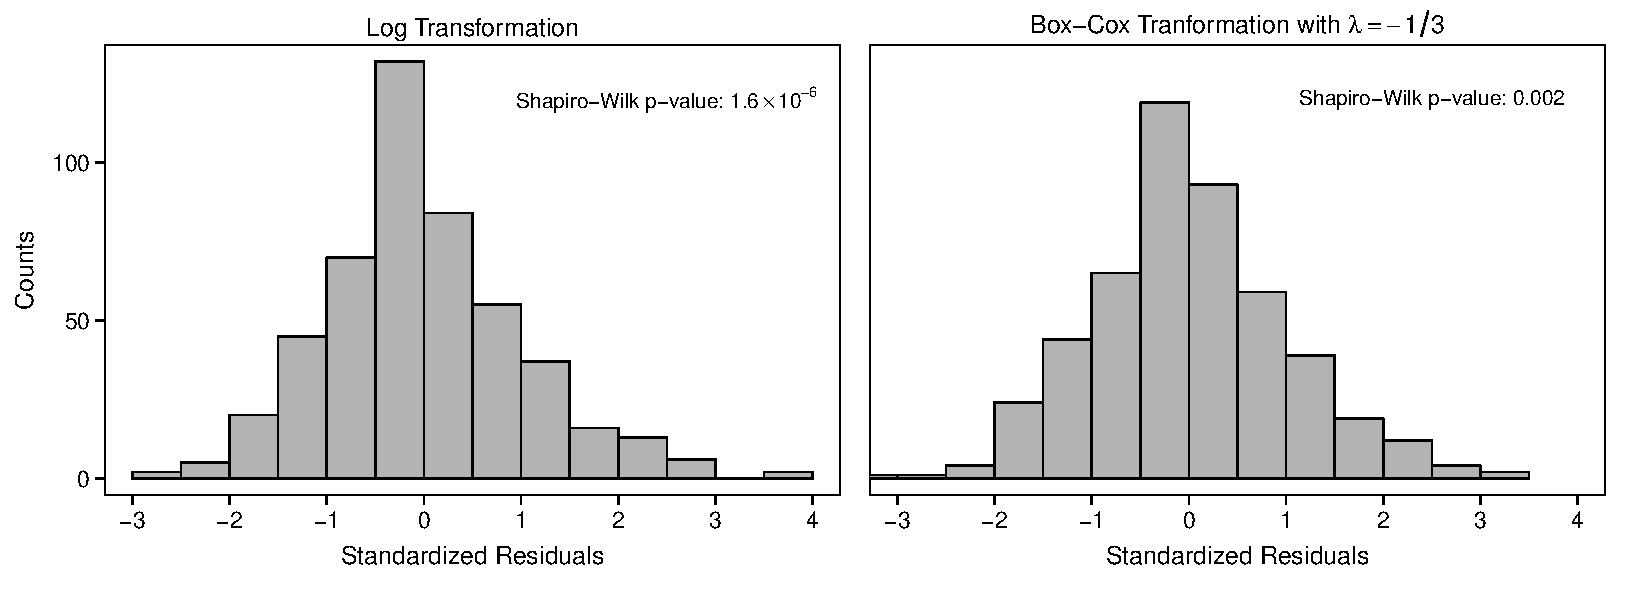
\includegraphics[width = \textwidth]{figs/cg-trans-residuals-hist.pdf}
\caption{}\label{fig:cg-trans-residuals-hist}
\end{center}
\end{figure}

Figure \ref{fig:cg-trans-qq-plot} shows the QQ plot for these residuals. The left panel confirms that a right-skew remains after the log-transformation, as suggested by the histogram in the left panel of Figure \ref{ig:cg-trans-residuals-hist}. The right panel of Figure \ref{ig:cg-trans-qq-plot} confirms that the Box-Cox transformation removes much or all of this skew, as suggested by the right panel of Figure \ref{ig:cg-trans-residuals-hist}. 

Although the Box-Cox transformation removes much or all of the skew, the residuals retain tails that are slightly heavier than the tails of the normal distribution. Notice that the data tend to have larger positive and larger negative quantiles than one would expect under a normal distribution. This suggests the residuals have a heavy tail, perhaps resembling a $t$ distribution with degrees of freedom in the rand 6 to 12. This also suggests that least squares might not be the most efficient estimator, even after transformation. Indeed, even after the Box-Cox transformation, the Shapiro-Wilk test rejects the null hypothesis of normality with $p = 0.002$. Assuming that these residuals follow a $t$-distribution, we can estimate the degrees of freedom using maximum likelihood estimate. This points toward a $t$ distribution with about 10 degrees of freedom. Recall that the biweight estimator is a (slightly) more efficient estimator for $t_{10}$ distributed errors. However, the least squares estimates \textit{assumes} normally distributed errors and thus the residuals might actually have heavier tails than this analysis suggests.

\begin{figure}[h!]
\begin{center}
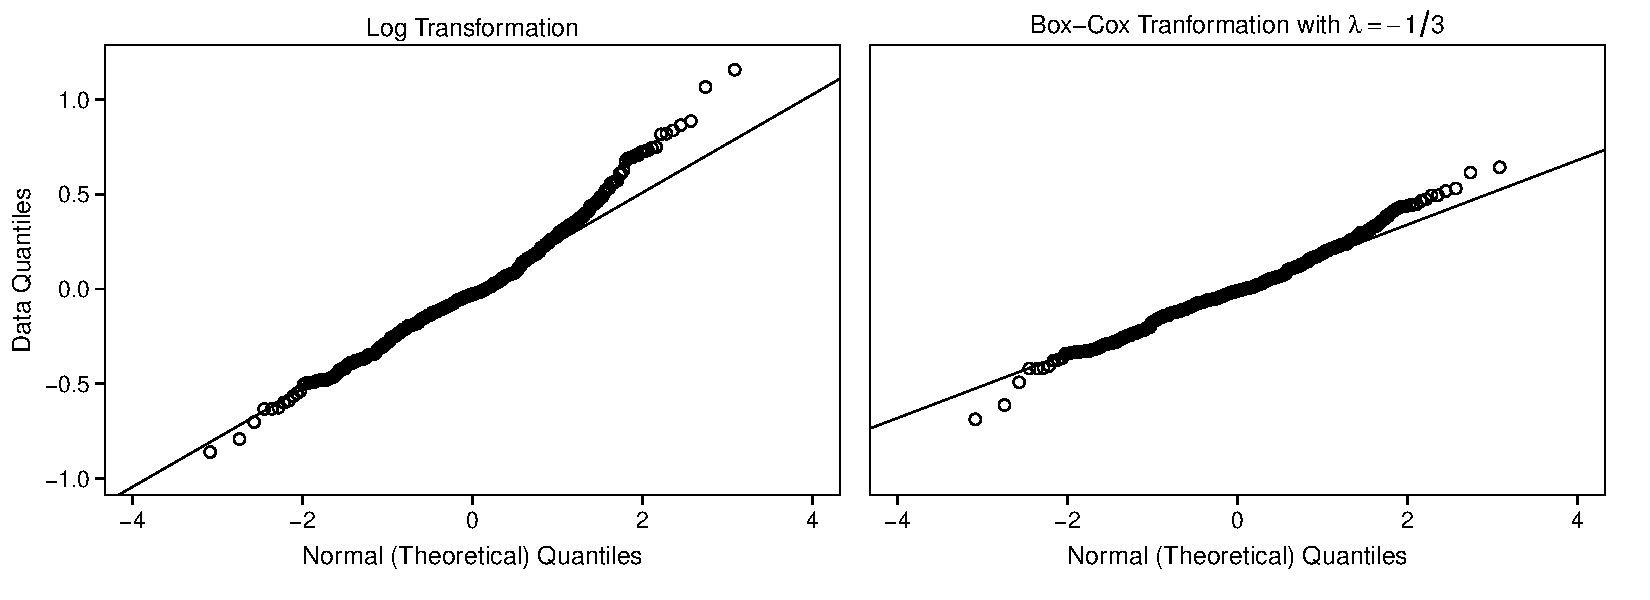
\includegraphics[width = \textwidth]{figs/cg-trans-qq-plot.pdf}
\caption{}\label{fig:cg-trans-qq-plot}
\end{center}
\end{figure}

After the Box-Cox transformation, the residuals are well-behaved. They are highly symmetric and only slightly heavy-tailed. In spite of nearly ideal situation, the simulations in Tables \ref{tab:mc-sims-100} and \ref{tab:mc-sims-1000} and Figure \ref{fig:mc-sims} suggest that the biweight estimate is a slightly better estimator. However, these differences are slight so it can be valuable to carefully examine examine both models--one that tries to fit all the data well and another that tries to fit most of the data well. 

%Table \ref{tab:cg-coef-tab} presents the coefficient estimate and confidence intervals, creating using the cluster-robust bootstrap recommend by Harden and Desmarais (????). The coefficients for the transformed and untransformed outcomes are not comparable, since the outcome is rescaled. The first column of Table \ref{tab:cg-coef-tab} uses Clark and Golder's approach (except for the bootstrapped confidence intervals). Notice that the interaction term $ENEG $\times$ log(Magnitude)$ is large and almost significant in Clark and Golder's model. 


%\begin{table}
%\begin{center}
%{\scriptsize
%
\begin{tabular}{l c c c c }
\hline
                                           & \specialcell{Least Squares\\w/ No Transformation} & \specialcell{Biweight\\w/ No Transformation} & \specialcell{Least Squares\\w/ Box-Cox Transformation} & \specialcell{Biweight\\w/Box-Cox Transformation} \\
\hline
Constant                                   & $1.92^{*}$        & $1.46^{*}$        & $0.87^{*}$        & $0.81^{*}$        \\
                                           & $[1.31;\ 2.58]$   & $[0.99;\ 2.25]$   & $[0.74;\ 0.99]$   & $[0.70;\ 0.99]$   \\
ENEG                                       & $0.11$            & $0.26$            & $0.02$            & $0.05$            \\
                                           & $[-0.17;\ 0.37]$  & $[-0.09;\ 0.44]$  & $[-0.03;\ 0.07]$  & $[-0.02;\ 0.08]$  \\
log(Magnitude)                             & $0.08$            & $0.49$            & $0.05$            & $0.07$            \\
                                           & $[-0.50;\ 0.43]$  & $[-0.23;\ 0.84]$  & $[-0.04;\ 0.11]$  & $[-0.03;\ 0.16]$  \\
Upper-Tier Seats                           & $-0.06$           & $-0.06$           & $0.00$            & $0.00$            \\
                                           & $[-0.11;\ 0.05]$  & $[-0.10;\ 0.03]$  & $[-0.01;\ 0.01]$  & $[-0.01;\ 0.01]$  \\
Presidential Candidates                    & $0.26$            & $0.17$            & $0.02$            & $0.03$            \\
                                           & $[-0.02;\ 0.51]$  & $[-0.30;\ 0.37]$  & $[-0.02;\ 0.06]$  & $[-0.06;\ 0.06]$  \\
Proximity                                  & $-3.10^{*}$       & $-2.88^{*}$       & $-0.52^{*}$       & $-0.54^{*}$       \\
                                           & $[-3.93;\ -2.25]$ & $[-3.76;\ -2.05]$ & $[-0.66;\ -0.38]$ & $[-0.70;\ -0.37]$ \\
ENEG $\times$ log(Magnitude)               & $0.26^{*}$        & $-0.03$           & $0.02$            & $0.01$            \\
                                           & $[0.01;\ 0.71]$   & $[-0.26;\ 0.55]$  & $[-0.01;\ 0.09]$  & $[-0.04;\ 0.09]$  \\
ENEG $\times$ Upper-Tier Seats             & $0.06$            & $0.06$            & $0.01$            & $0.01$            \\
                                           & $[-0.03;\ 0.09]$  & $[-0.01;\ 0.09]$  & $[0.00;\ 0.01]$   & $[0.00;\ 0.01]$   \\
Presidential Candidates $\times$ Proximity & $0.68^{*}$        & $0.71^{*}$        & $0.13^{*}$        & $0.13^{*}$        \\
                                           & $[0.33;\ 1.11]$   & $[0.39;\ 1.31]$   & $[0.07;\ 0.21]$   & $[0.07;\ 0.25]$   \\
\hline
Num. obs.                                  & 487               & 487               & 487               & 487               \\
\hline
\multicolumn{5}{l}{\scriptsize{$^*$ 0 outside the confidence interval}}
\end{tabular}

%}
%\caption{Coefficients estimated using least squares and biweight estimators, with and without the Box-Cox transformation. The first column replications Clark and Golder's (2006) Table 2, column 6, except using cluster-bootstrap confidence intervals. The remaining models make an attempt to address the skewednd/or heavy-tailed residuals. Notice that simply transforming the outcome to be more consistent with the assumed model and/or using the more robust biweight estimator substantial reduces the evidence for their hypothesis.}\label{tab:cg-coef-tab}
%\end{center}
%\end{table}

Figure \ref{fig:cg-fd-plots} plots the effect of increasing social heterogenty from ENEP = 1.06 (10th percentile) to ENEP = 2.48 (90th percentile) as the district magnitude varies. Note the the effect of district magnitude is nonlinear because it is logged in the regression model but unlogged along the horizontal axis. The upper-left figure replicates Clark and Golder's approach (except of the cluster-bootstrap confidence intervals) and replicates their finding, which they summarize:

\begin{quote}
[These results] clearly illustrate that in established democracies, ethnic heterogeneity significantly increases the number of parties once the electoral system is sufficiently permissive. This is exactly what Duverger?s theory predicts. To be more specific, Figure 1a [our upper-left panel of Figure \ref{fig:cg-fd-plots}], based on the pooled model with established democracies, indicates that ethnic heterogeneity will increase the number of electoral parties once we move beyond nonpermissive electoral systems with single-member districts?when [Magnitude = 1].
\end{quote}

But this evidence breaks down once we account for the non-normality of the errors. The lower-left panel of Figure \ref{fig:cg-fd-plots} shows that simply using the biweight estimator as a robust alternative to least squares produces estimated interaction in the \text{opposite} direction as the hypothesis predicts, though small and not statistically significant. The upper-right panel of Figure \ref{fig:cg-fd-plots} shows that simply transforming the outcome variable to make the data more consistent with the assumed normal-linear model substantially reduces the estimated effect across the range of district magnitude to a statistically insignificant, negligible effect.

However, we argue that the best approach for these data is to transform the outcome variable to obtain a roughly symmetric error distribution and use the biweight estimator to handle the remaining heavy tails shown in the left panel of Figure \ref{fig:cg-trans-qq-plot}. Notice that this approach reduces effect of social heterogeneity to nearly zero and suggests that these data offer very little evidence for interaction consistent with the hypothesis.

\begin{figure}[h!]
\begin{center}
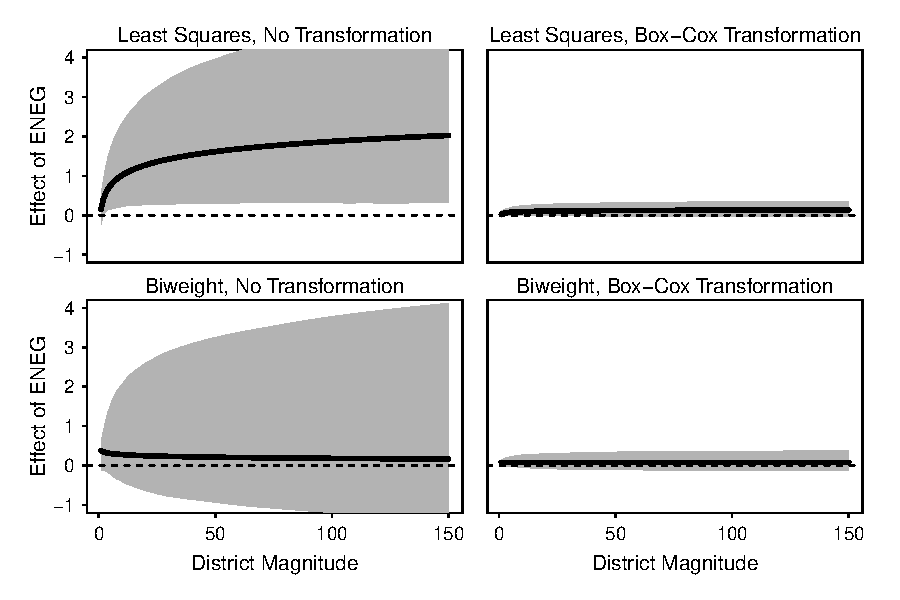
\includegraphics[scale = 0.8]{figs/cg-fd-plots.pdf}
\caption{}\label{fig:cg-fd-plots}
\end{center}
\end{figure}

Because the scale of the estimates differ drastically across the choice to transform the outcome variable or not, we present the relevant quantities of interest in Table \ref{tab:cg-qi}. In this case, we are interested in the effect of substantially increasing social heterogeneity from ENEP = 1.06 (10th percentile) to ENEP = 2.48 (90th percentile) on the median number of political parties when district magnitude is one and also when district magnitude is 14. Since the hypothesis suggests that this effect should be larger when the district magnitude is larger, we are also interested in the difference between these two effects. For simplicity, we simply focus our discussion on the differences between the typical approach, least squares with no transformation, and the approach we recommend, robust estimation after transformation.

The first row of Table \ref{tab:cg-qi} suggest that in countries with single-member districts, a substantial increase in ENEG (10th to 90th percentile) increases the median ENEP by about 0.16 [-0.24; 0.53] parties. On the other hand, in large, multimember districts (magnitude of 14), the same increase in social heterogeneity increases the ENEP by about 1.14 [0.26; 2.67] parties. This is just as the hypothesis predicts. Further, this increase of 0.98 [0.06; 2.65] is large and statistically significant.

However, once we make an effort to account for the non-normality of the residuals by transforming the outcome variable and using the robust biweight estimator, this evidence for substantial interaction simply disappears. These estimates suggest that, in single-member districts, a substantial increase in social heterogeneity increases the median ENEP by about 0.08 [-0.04; 0.15] parties--about half the initial estimate of Clark and Golder. In large, multimember districts (magnitude of 14), the effect again shrinks to 0.08 [-0.06; 0.28]--about 7\% of Clark and Golder's intial estimate. This leads to an estimated increase of 0.00 [-0.17; 0.25] in the effect of social heterogeneity as we move from single-member districts to large, multimember districts. 

Clark and Golder adopt the convention of many researchers in political science--taking least squares estimates at face value without thinking carefully about the distribution of the errors. Indeed, the Gauss-Markov theorem encourages this convention by noting that least squares is the \textit{best} linear unbiased estimator. However, we argue that the restriction to linear estimators is unnecessary and counter-productive. By taking advantage of transformations to make the errors more consistent with the normal-linear model (approximately normal or at least symmetric) and using robust estimators if necessary to deal with remaining heavy tails, we show that we can reach different conclusions. 

[Discuss the residuals from the transformed models.]

\begin{table}
{\scriptsize
% quantreg::latex.table(x = qitab, file = "doc/tabs/cg-qi", rowlabel = "",      rowlabel.just = "l", cgroup = c("First-Difference When \\textit{M} = 1",          "First-Difference When \\textit{M} = 14", "Second-Difference"),      rgroup = c("No Transformation", "Box-Cox Transformation"),      n.rgroup = c(2, 2), table.env = FALSE) 
%
\begin{center}
\begin{tabular}{|l||c|c||c|c||c|c|} \hline
\multicolumn{1}{|l||}{\bf }&\multicolumn{2}{c||}{\bf First-Difference When \textit{M} = 1}&\multicolumn{2}{c||}{\bf First-Difference When \textit{M} = 14}&\multicolumn{2}{c|}{\bf Second-Difference}\\ \cline{2-7}
\multicolumn{1}{|l||}{}&\multicolumn{1}{c|}{Est.}&\multicolumn{1}{c||}{90\% CI}&\multicolumn{1}{c|}{Est.}&\multicolumn{1}{c||}{90\% CI}&\multicolumn{1}{c|}{Est.}&\multicolumn{1}{c|}{90\% CI}\\ \hline
{\bf No Transformation}&&&&&&\\
~~Least Squares&~~~~~0.16~~~~~&[-0.24;~~0.53]&~~~~~1.14~~~~~&[0.26;~2.67]~~&~~~~~0.98~~~~~&[0.06;~2.65]~~\\ 
~~Biweight&~~~~~0.37~~~~~&[-0.12;~~0.62]&~~~~~0.26~~~~~&[-0.51;~~2.33]&~~~~~-0.11~~~~&[-0.96;~~2.05]\\ \hline
{\bf Box-Cox Transformation}&&&&&&\\
~~Least Squares&~~~~~0.03~~~~~&[-0.05;~~0.12]&~~~~~0.10~~~~~&[0.00;~0.26]~~&~~~~~0.07~~~~~&[-0.07;~~0.26]\\ 
~~Biweight&~~~~~0.08~~~~~&[-0.04;~~0.15]&~~~~~0.08~~~~~&[-0.06;~~0.28]&~~~~~0.00~~~~~&[-0.17;~~0.25]\\ 
\hline
\end{tabular}
\end{center}

}
\caption{Quantities of interest from least squares and biweight estmates, with and without the Box-Cox transformation of the outcome variable. Notice that the least squares estimates without transforming the outcome variable are consistent with Clark and Golder's hypothesis. However, using the robust biweight estimator,  transforming the outcome variable, or both substantially reduce the amount of evidence that these data offer in favor of the hypothesis. In particular, the biweight estimator suggests that social heterogeneity has small, substantively insignificant effects regardless of the electoral rules. Indeed, the effect is, \textit{at most}, about 1/5 of of a political party per ethnic group, with a estimate of about 1/20 of a political party per ethnic group. }\label{tab:cg-qi}
\end{table}

We offer a different approach than most applied research in political science adopts in practice. Rather than relying on the artificial Gauss-Markov theorem and BLUE estimators, we suggest that careful consideration of residual is very important. We have shown that can be tremendous gains in efficiency by using robust estimators in the face of heavy-tailed error distributions, and we have shown that our approach leads to different conclusions than Clark and Golder (2006). But the approach we advocate is not powerful because it gives different results. It is powerful because it is substantively informative. Below we discuss several \textit{substantive} points that one can take from our brief analysis of Clark and Golder's data.
\begin{itemize}
\item \textit{Perhaps Duverger's logic is not as well-supported empirically as the literature would suggest.} Indeed, the evidence offered by the normal linear model seems to hinge on a few cases that seem inconsistent with the majority of the data. However, rejection of Duverger's theory or Clark and Golder's (2006) analysis is premature for three reasons. First, the theoretical logic for Duverger's hypotheses is clear and compelling (CITES). Second, many studies beyond Clark and Golder (2006), including experimental work, find substantial empirical support for the hypotheses. Finally, the biweight $M$-estimator suggests several potential shortcomings in terms of theory and measures that might currently undermine the evidence for these theories.
\item \textit{Room for improvement exists in the measurement of ``established democracies.''}
\item \textit{Room for improvement exists in the measurement of ``social heterogeneity.''}
\item \textit{We need a stronger theory about the dynamics with which systems reach an equilibrium number of parties.}
\item \textit{We need additional research into how systems respond to the introduction of additional parties into formerly authoritarian, single-party systems.}
\end{itemize}

\singlespace
\bibliographystyle{apsr_fs}
%\bibliography{/Users/carlislerainey/Dropbox/papers/bibliography/bibliography.bib}
\bibliography{/Users/rcrainey/Dropbox/papers/bibliography/bibliography.bib}


\newpage
\doublespace
\begin{appendix}
\begin{center}
\textbf{{\LARGE Appendix}}\\\vspace{2mm}
\textbf{{\large The Heavy Tails of Electoral Data}}\\\vspace{2mm}

\end{center}
\section{}


\end{appendix}


\end{document}